\documentclass[]{article}

\usepackage[top=2cm, bottom=2.5cm, left=2.0cm, right=2.0cm]{geometry}
\usepackage{xcolor}
\usepackage{tikz}
\usepackage{pgfplots}
\usepackage{algorithm}
\usepackage{algorithmic}
\usepackage{appendix}
\usepackage{placeins}

\newlength{\xdim}

\definecolor{calculate}{HTML}{D7191C}
\definecolor{copyBack}{HTML}{FDAE61}

%opening
\title{Multiprocessor Systems - Assignment II (pthread)}
\author{Adrian Holfter, Lucie Labadie}

\begin{document}

\maketitle

\section{How to run}

\paragraph{} The archive contains a \emph{Makefile}. Running \texttt{make} in the directory will create a binary, \texttt{gaussian\_par}.

\section{Implementation}

\subsection{Pthread-based Gaussian parallelization}

\paragraph{} Based on the provided sequential implementation of gaussian elimination for linear equation systems, we created a parallelized version using \emph{pthread}.

\paragraph{} The data distribution is done in a \emph{cyclic row-wise} manner, meaning that rows are assigned to processors using round-robin, rather than assigning blocks of rows to each processor. This is to account for the decreasing amount of work needed for rows further down in the equation system; in a block-wise fashion there would be a load imbalance. The cyclic distribution is achieved by giving each thread an initial row offset and the total number of workers as step size.

\paragraph{} We restructured the implementation a bit in a way that a thread will always be responsible for one row at a time. While doing the calculation work for one row, the thread may read values from other rows, but it will only write in the currently assigned row.

\paragraph{} Each thread will first carry out the elimination step for its row using the division result of each of the previous rows. This requires all previous rows to have finished the division step. If this step is not done yet, the thread will wait. Once this is done, the division step will be carried out for the assigned row.

\paragraph{} To know if a previous row finished its elimination, there is a global table containing a flag for every row ($1$ if division step is finished, $0$ if not). As soon as the division step is finished for the previous rows, a thread can execute the elimination step on its own row and then continue with the division. Then the corresponding flag in the table is changed from $0$ to $1$. All writing and reading in the flag table is protected by a mutex.

\paragraph{} We used one global condition variable to implement the waiting for the completion of a row. As soon as a row is completely finished and the corresponding flag is set in the table, all waiting threads are woken up to re-evaluate their waiting condition (checking a flag in the flag table). This means that a waiting thread will be woken up by \emph{any} finished row, not only by the one it is waiting for. However, we thought this is still more elegant than having one condition variable per row.

\section{Measurements}

The measurements were taken on the \emph{kraken.tek.bth.se} Server. The executables were compiled with the \texttt{-O2} option, to enable compiler optimizations. Measurement was done using the bash-builtin \texttt{time} command. Every measurement was taken 10 times and the smallest value was used to account for background load and operating system caches.

\subsection{Pthread-based Gaussian elimination}

Table \ref{tab:gauss-runtime} shows the runtimes of the different versions of the row-based gaussian elimination. Figure \ref{fig:gauss-chart} also visualizes this.

\begin{figure}[h]
	\centering
	\begin{tabular}{|l|r|r|}
		\hline
		\textbf{Version} & \textbf{shortest runtime [s]} & \textbf{speedup} \\
		\hline
		Sequential single-threaded		& 11.37 & 1.00 \\ 
		\hline 
		pthread 1 thread				& 8.44 & 1.34 \\ 
		\hline 
		pthread 2 threads				& 5.05 & 2.25 \\ 
		\hline 
		pthread 4 threads 				& 3.06 & 3.71 \\ 
		\hline 
		pthread 8 threads				& 2.59 & 4.39 \\ 
		\hline 
	\end{tabular} 
	\caption{Runtime comparison for gaussian elimination}
	\label{tab:gauss-runtime}
\end{figure}

\begin{figure}[h]
	\centering
	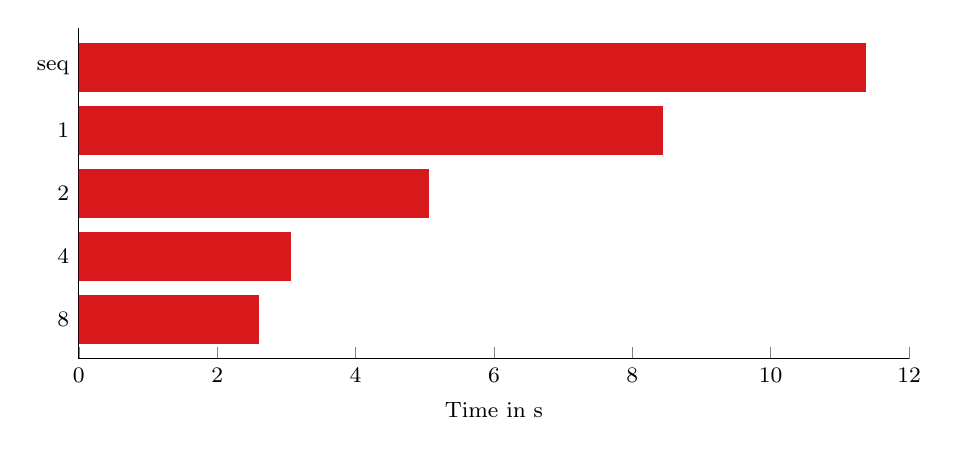
\begin{tikzpicture}
	\begin{axis}[
	xbar stacked,
	legend style={
		legend columns=4,
		at={(xticklabel cs:0.5)},
		anchor=north,
		draw=none
	},
	ytick=data,
	axis y line*=none,
	axis x line*=bottom,
	tick label style={font=\footnotesize},
	legend style={font=\footnotesize},
	label style={font=\footnotesize},
	xtick={0, 2.0, 4.0, 6.0, 8.0, 10.0, 12.0},
	width=1.0\textwidth,
	bar width=6mm,
	xlabel={Time in s},
	yticklabels={seq, 1, 2, 4, 8},
	xmin=0,
	xmax=12.0,
	area legend,
	y=8mm,
	enlarge y limits={abs=0.625},
	]
	\addplot[calculate,fill=calculate] coordinates
	{(11.37,4) (8.44,3) (5.05,2) (3.06,1) (2.59, 0)};
	\end{axis}  
	\end{tikzpicture}
	\caption{Runtime comparison chart for gaussian elimination}
	\label{fig:gauss-chart}
\end{figure}

As can be seen, we achieved a substantial speedup over the original single-threaded version.
Interestingly, our implementation is also considerably faster when using only one core than the provided sequential version.
This is most probably due to the changed order of computation: In the original version, after a division, the elimination step is carried out on all following rows. Then, the next division is carried out. In our implementation, the elimination of a row is done for all rows before it. After that, the division is done. So the order to dependent actions (division must be followed by elimination of subsequent rows) was kept and only the order of independent actions (order of eliminations) was changed.
We assume that our execution order is more cache-friendly than the original implementation.

\end{document}